\documentclass{article}
\usepackage{graphicx} % Required for inserting images

\begin{document}

\begin{titlepage}
    \centering
    
    \huge \textbf{Assignment 4}
    
    \vspace{5cm} 
    
    \Huge \textbf{General Theory of Relativity}

    \vspace{5cm}

    \Large \textbf{Deepak S}
    
    \vspace{2cm}
    
    \large \today

\end{titlepage}

\section{Introduction}

In 1907, two years after Einstein released his Special Theory of Relativity, he attempted to modify Newton's theory of gravitation to fit with his Special Theory of Relativity. In the Special Theory of Relativity, Einstein gave laws that govern the Time Dilation, Length Contraction, and Relativistic Addition of Velocities. 

\vspace{1cm}

\begin{flushleft}
\textbf{Time Dilation:} According to the theory, time is not absolute but relative to the observer's motion. Einstein derived the time dilation equation, which states that time passes more slowly for objects in motion relative to an observer at rest. The relationship between the time experienced by a moving object and the time experienced by an observer at rest can be expressed as:
\end{flushleft}

\[
\Delta t' = \frac{\Delta t}{\sqrt{1 - \frac{v^2}{c^2}}}
\]

\begin{flushleft}
where:\\
$\Delta t$ is the time interval measured by the observer at rest. \\
$\Delta t'$ is the time interval experienced by the moving object. \\
$v$ is the relative velocity between the observer and the moving object. \\
$c$ is the speed of light.
\end{flushleft}

\vspace{1cm}

\begin{flushleft}
\textbf{Length Contraction:} The theory also introduced the concept of length contraction, which describes how the length of an object changes when it is moving relative to an observer at rest. The relationship between the length observed by the moving object and the length observed by an observer at rest can be expressed as:
\end{flushleft}

\[
L' = \frac{L}{\sqrt{1 - \frac{v^2}{c^2}}}
\]

\begin{flushleft}
where:\\
$L$ is the length measured by the observer at rest. \\
$L'$ is the length observed by the moving object. \\
$v$ is the relative velocity between the observer and the moving object. \\
$c$ is the speed of light.
\end{flushleft}

\vspace{1cm}

\begin{flushleft}
\textbf{Relativistic Addition of Velocities:} The theory introduced a modified formula for adding velocities in relativistic scenarios. According to the Special Theory of Relativity, velocities do not simply add up but combine using a nonlinear equation known as the relativistic addition of velocities:
\end{flushleft}

\[
v' = \frac{v + u}{1 + \frac{vu}{c^2}}
\]

\begin{flushleft}
where:\\
$v$ is the velocity of an object relative to an observer. \\
$u$ is the velocity of a second object relative to the first object. \\
$v'$ is the relative velocity of the second object with respect to the observer. \\
$c$ is the speed of light.
\end{flushleft}

\vspace{0.25cm}

\begin{flushleft}
\textbf{\underline{Connection between Special and General Theory of Relativity}}
\end{flushleft}

\vspace{0.25cm}
\begin{flushleft}
The General Theory of Relativity, conceived by the brilliant mind of Albert Einstein in 1915, ushered in a new era of understanding gravity, spacetime, and the enigmatic universe we inhabit. This groundbreaking theory revolutionized our perception of gravity, transforming it from a mere force of attraction to a profound interplay between the geometry of spacetime and the presence of matter and energy.
\end{flushleft}
\vspace{0.5cm}
\setlength{\parindent}{0em}
\textbf{Concepts presented by this theory are:}
\vspace{0.5cm}
\begin{flushleft}
\textbf{Curvature of Spacetime:} In Einstein's General Theory of Relativity, gravity is depicted as the curvature of spacetime caused by massive objects. As though creating a cosmic divot, the presence of matter and energy bends the very fabric of spacetime, shaping the paths that objects traverse.
\end{flushleft}

\[
G_{\mu\nu} = 8\pi T_{\mu\nu}
\]

\vspace{0.5cm}

\begin{flushleft}
\textbf{Unity of Gravitational and Inertial Forces:} The Equivalence Principle lies at the heart of Einstein's theory, forging a profound connection between gravitational and inertial forces. It suggests that the effects of gravity experienced by an observer are indistinguishable from those experienced in an accelerated frame of reference.
\end{flushleft}

\[
R_{\mu\nu} - \frac{1}{2} R g_{\mu\nu} = \frac{8\pi G}{c^4} T_{\mu\nu}
\]

\vspace{0.5cm}
\begin{figure}[h]
\centering
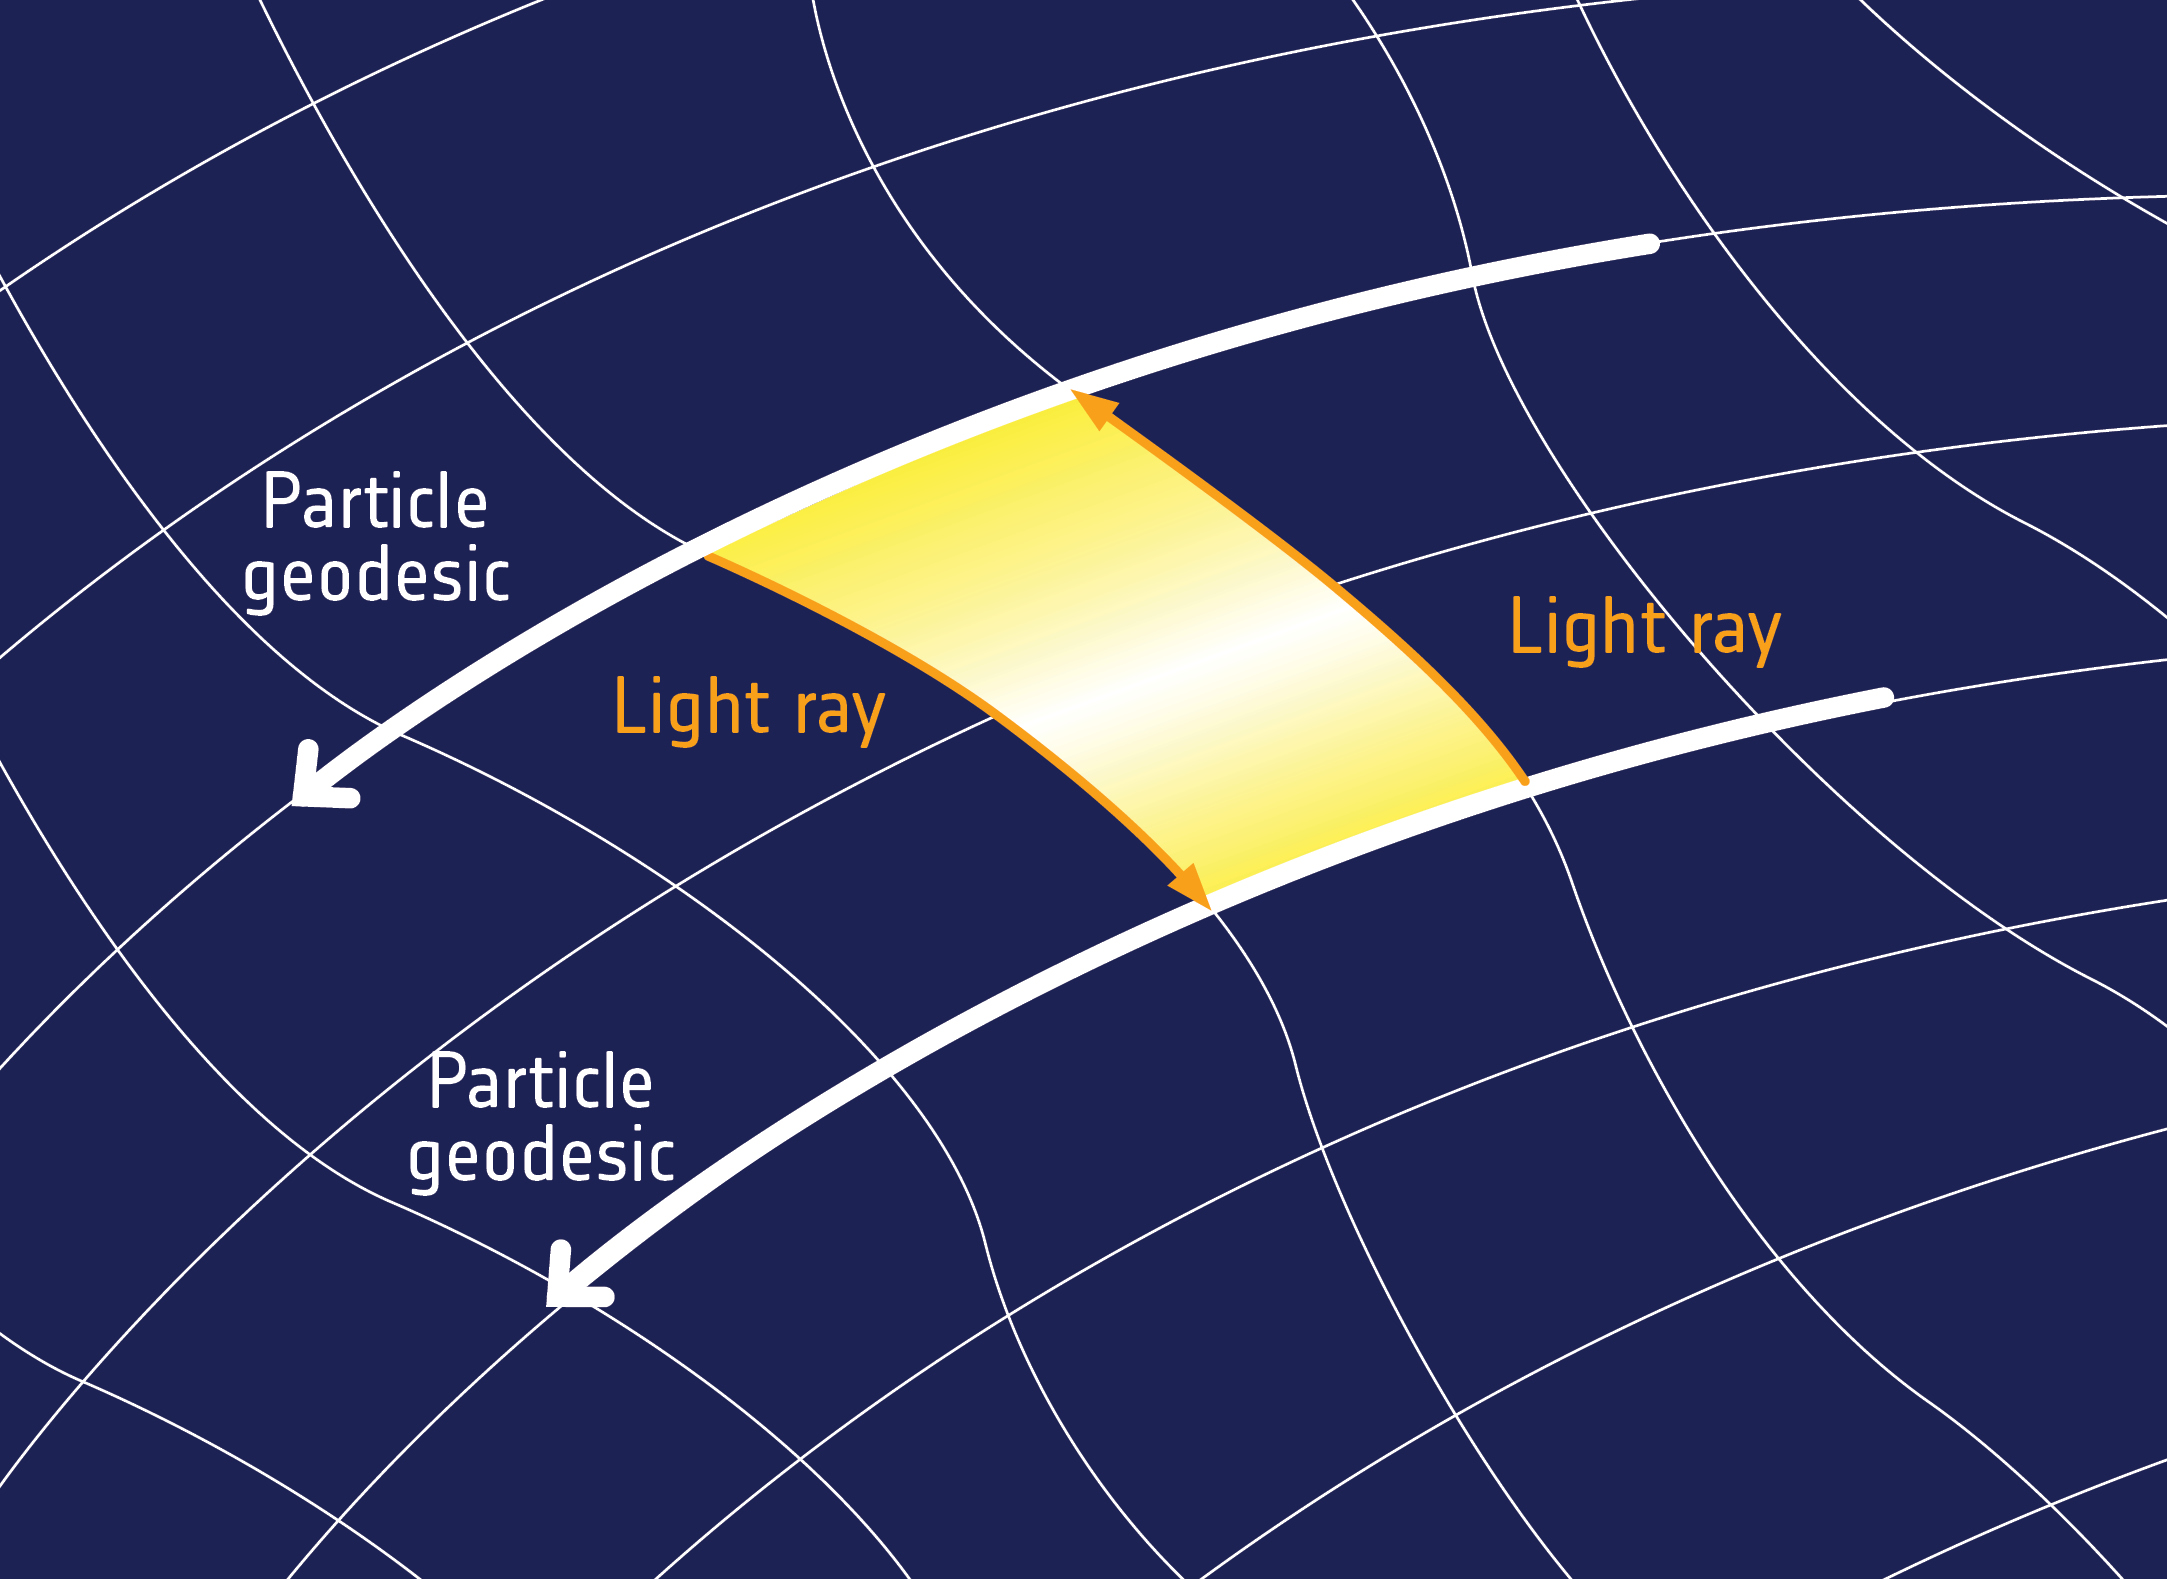
\includegraphics[width=0.7\textwidth]{Measuring_spacetime_curvature.jpg}
\caption{Visualization of spacetime curvature caused by a massive object}
\label{fig:spacetime_curvature}
\end{figure}
\vspace{0.5cm}

\begin{flushleft}
\textbf{Geodesic Motion:} Within the General Theory of Relativity, objects move along geodesics, which can be envisioned as the most efficient paths through the curved spacetime. Similar to a hiker following the natural contours of a landscape, objects in free fall follow these geodesic paths, appearing to move in straight lines within the curved geometry.
\end{flushleft}

\[
\frac{d^2 x^\mu}{d\tau^2} + \Gamma^\alpha_{\beta\mu} \frac{dx^\alpha}{d\tau} \frac{dx^\beta}{d\tau} = 0
\]

\vspace{0.5cm}

\begin{flushleft}
\textbf{Relativistic Effects:} The theory encapsulates the remarkable effects of Special Relativity, including time dilation and length contraction. As objects move relative to one another, time appears to pass at different rates, and lengths along the direction of motion appear to contract. These phenomena unveil the intricate interplay of motion, gravity, and spacetime, revealing the captivating nature of our universe.
\end{flushleft}

\[
\Delta t' = \frac{\Delta t}{\sqrt{1 - \frac{v^2}{c^2}}}
\]

\[
L' = \frac{L}{\sqrt{1 - \frac{v^2}{c^2}}}
\]



\section{Conclusion}

In conclusion, the General Theory of Relativity revolutionized our understanding of gravity, unveiling a profound connection between the geometry of spacetime and the distribution of matter and energy. By extending the principles of Special Relativity to include accelerated frames and gravitational forces, Einstein's theory provided a comprehensive framework for describing the curvature of spacetime, the unity of gravitational and inertial forces, geodesic motion, and relativistic effects. The General Theory of Relativity has withstood the test of time and continues to be a cornerstone of modern physics, influencing numerous scientific endeavors and furthering our exploration of the cosmos.

\vspace{1cm}

\textbf{Motivation to write about General Theory of Relativity}

I chose to explore the General Theory of Relativity for my report due to its profound impact on our understanding of the universe. The theory, developed by Albert Einstein, revolutionized our perception of gravity by presenting a new perspective that connects the curvature of spacetime with the presence of matter and energy. This interplay between geometry and gravity fascinated me and motivated me to delve deeper into the subject.

\vspace{0.5cm}
\textbf{References:}
\begin{enumerate}
  \item Wudka, J. (2016). General Relativity and Cosmology. University of California, Riverside. Retrieved from \textit{https://iontrap.umd.edu/wp-content/uploads/2016/01\\/WudkaGR-7.pdf}.
  \item Einstein, A. (1916). Relativity: The Special and the General Theory. Retrieved from \textit{https://www.ncjindalps.com/pdf/PHYSICS/Relativity\%20The\%20Special\\\%20and\%20the\%20General\%20Theory\%20-\%20Albert\%20Einstein.pdf}.
\end{enumerate}

\vspace{1cm}

\textbf{GitHub Repository:} My report and code can be found in my GitHub repository: \textit{https://github.com/mm22b011-deepaks}

\end{document}
